\documentclass[]{article}
\usepackage{lmodern}
\usepackage{amssymb,amsmath}
\usepackage{ifxetex,ifluatex}
\usepackage{fixltx2e} % provides \textsubscript
\ifnum 0\ifxetex 1\fi\ifluatex 1\fi=0 % if pdftex
  \usepackage[T1]{fontenc}
  \usepackage[utf8]{inputenc}
\else % if luatex or xelatex
  \ifxetex
    \usepackage{mathspec}
  \else
    \usepackage{fontspec}
  \fi
  \defaultfontfeatures{Ligatures=TeX,Scale=MatchLowercase}
\fi
% use upquote if available, for straight quotes in verbatim environments
\IfFileExists{upquote.sty}{\usepackage{upquote}}{}
% use microtype if available
\IfFileExists{microtype.sty}{%
\usepackage{microtype}
\UseMicrotypeSet[protrusion]{basicmath} % disable protrusion for tt fonts
}{}
\usepackage[margin=1in]{geometry}
\usepackage{hyperref}
\hypersetup{unicode=true,
            pdftitle={razzo pipeline},
            pdfauthor={Giovanni Laudanno and Richel J.C. Bilderbeek},
            pdfborder={0 0 0},
            breaklinks=true}
\urlstyle{same}  % don't use monospace font for urls
\usepackage{color}
\usepackage{fancyvrb}
\newcommand{\VerbBar}{|}
\newcommand{\VERB}{\Verb[commandchars=\\\{\}]}
\DefineVerbatimEnvironment{Highlighting}{Verbatim}{commandchars=\\\{\}}
% Add ',fontsize=\small' for more characters per line
\usepackage{framed}
\definecolor{shadecolor}{RGB}{248,248,248}
\newenvironment{Shaded}{\begin{snugshade}}{\end{snugshade}}
\newcommand{\KeywordTok}[1]{\textcolor[rgb]{0.13,0.29,0.53}{\textbf{#1}}}
\newcommand{\DataTypeTok}[1]{\textcolor[rgb]{0.13,0.29,0.53}{#1}}
\newcommand{\DecValTok}[1]{\textcolor[rgb]{0.00,0.00,0.81}{#1}}
\newcommand{\BaseNTok}[1]{\textcolor[rgb]{0.00,0.00,0.81}{#1}}
\newcommand{\FloatTok}[1]{\textcolor[rgb]{0.00,0.00,0.81}{#1}}
\newcommand{\ConstantTok}[1]{\textcolor[rgb]{0.00,0.00,0.00}{#1}}
\newcommand{\CharTok}[1]{\textcolor[rgb]{0.31,0.60,0.02}{#1}}
\newcommand{\SpecialCharTok}[1]{\textcolor[rgb]{0.00,0.00,0.00}{#1}}
\newcommand{\StringTok}[1]{\textcolor[rgb]{0.31,0.60,0.02}{#1}}
\newcommand{\VerbatimStringTok}[1]{\textcolor[rgb]{0.31,0.60,0.02}{#1}}
\newcommand{\SpecialStringTok}[1]{\textcolor[rgb]{0.31,0.60,0.02}{#1}}
\newcommand{\ImportTok}[1]{#1}
\newcommand{\CommentTok}[1]{\textcolor[rgb]{0.56,0.35,0.01}{\textit{#1}}}
\newcommand{\DocumentationTok}[1]{\textcolor[rgb]{0.56,0.35,0.01}{\textbf{\textit{#1}}}}
\newcommand{\AnnotationTok}[1]{\textcolor[rgb]{0.56,0.35,0.01}{\textbf{\textit{#1}}}}
\newcommand{\CommentVarTok}[1]{\textcolor[rgb]{0.56,0.35,0.01}{\textbf{\textit{#1}}}}
\newcommand{\OtherTok}[1]{\textcolor[rgb]{0.56,0.35,0.01}{#1}}
\newcommand{\FunctionTok}[1]{\textcolor[rgb]{0.00,0.00,0.00}{#1}}
\newcommand{\VariableTok}[1]{\textcolor[rgb]{0.00,0.00,0.00}{#1}}
\newcommand{\ControlFlowTok}[1]{\textcolor[rgb]{0.13,0.29,0.53}{\textbf{#1}}}
\newcommand{\OperatorTok}[1]{\textcolor[rgb]{0.81,0.36,0.00}{\textbf{#1}}}
\newcommand{\BuiltInTok}[1]{#1}
\newcommand{\ExtensionTok}[1]{#1}
\newcommand{\PreprocessorTok}[1]{\textcolor[rgb]{0.56,0.35,0.01}{\textit{#1}}}
\newcommand{\AttributeTok}[1]{\textcolor[rgb]{0.77,0.63,0.00}{#1}}
\newcommand{\RegionMarkerTok}[1]{#1}
\newcommand{\InformationTok}[1]{\textcolor[rgb]{0.56,0.35,0.01}{\textbf{\textit{#1}}}}
\newcommand{\WarningTok}[1]{\textcolor[rgb]{0.56,0.35,0.01}{\textbf{\textit{#1}}}}
\newcommand{\AlertTok}[1]{\textcolor[rgb]{0.94,0.16,0.16}{#1}}
\newcommand{\ErrorTok}[1]{\textcolor[rgb]{0.64,0.00,0.00}{\textbf{#1}}}
\newcommand{\NormalTok}[1]{#1}
\usepackage{longtable,booktabs}
\usepackage{graphicx,grffile}
\makeatletter
\def\maxwidth{\ifdim\Gin@nat@width>\linewidth\linewidth\else\Gin@nat@width\fi}
\def\maxheight{\ifdim\Gin@nat@height>\textheight\textheight\else\Gin@nat@height\fi}
\makeatother
% Scale images if necessary, so that they will not overflow the page
% margins by default, and it is still possible to overwrite the defaults
% using explicit options in \includegraphics[width, height, ...]{}
\setkeys{Gin}{width=\maxwidth,height=\maxheight,keepaspectratio}
\IfFileExists{parskip.sty}{%
\usepackage{parskip}
}{% else
\setlength{\parindent}{0pt}
\setlength{\parskip}{6pt plus 2pt minus 1pt}
}
\setlength{\emergencystretch}{3em}  % prevent overfull lines
\providecommand{\tightlist}{%
  \setlength{\itemsep}{0pt}\setlength{\parskip}{0pt}}
\setcounter{secnumdepth}{0}
% Redefines (sub)paragraphs to behave more like sections
\ifx\paragraph\undefined\else
\let\oldparagraph\paragraph
\renewcommand{\paragraph}[1]{\oldparagraph{#1}\mbox{}}
\fi
\ifx\subparagraph\undefined\else
\let\oldsubparagraph\subparagraph
\renewcommand{\subparagraph}[1]{\oldsubparagraph{#1}\mbox{}}
\fi

%%% Use protect on footnotes to avoid problems with footnotes in titles
\let\rmarkdownfootnote\footnote%
\def\footnote{\protect\rmarkdownfootnote}

%%% Change title format to be more compact
\usepackage{titling}

% Create subtitle command for use in maketitle
\newcommand{\subtitle}[1]{
  \posttitle{
    \begin{center}\large#1\end{center}
    }
}

\setlength{\droptitle}{-2em}
  \title{razzo pipeline}
  \pretitle{\vspace{\droptitle}\centering\huge}
  \posttitle{\par}
  \author{Giovanni Laudanno and Richel J.C. Bilderbeek}
  \preauthor{\centering\large\emph}
  \postauthor{\par}
  \predate{\centering\large\emph}
  \postdate{\par}
  \date{2018-11-01}


\begin{document}
\maketitle

Legenda: nLTT = normalized lineages through time; BD = Birth Death
Model; MBD = Multiple Birth Death Model;

This is the pipeline to follow for the Razzo project. Our aim is to
compare two nLTT distributions related to two tree posteriors: one
descending from MBD alignments and another one from BD alignments. Both
posteriors are generated using a BD prior in BEAST.

\subsection{Folder structure}\label{folder-structure}

In \texttt{razzo\_project}, there is a folder called \texttt{data}. In
\texttt{data}, there are folders named after their parameters, e.g.
\texttt{0.2-0.15-1-0.1}. In each of these folders, there are folders
named after their seeds, e.g. \texttt{1}. In each of these folders,
there are:

\begin{longtable}[]{@{}lll@{}}
\toprule
\begin{minipage}[b]{0.16\columnwidth}\raggedright\strut
Filename\strut
\end{minipage} & \begin{minipage}[b]{0.45\columnwidth}\raggedright\strut
Description\strut
\end{minipage} & \begin{minipage}[b]{0.30\columnwidth}\raggedright\strut
Created by\strut
\end{minipage}\tabularnewline
\midrule
\endhead
\begin{minipage}[t]{0.16\columnwidth}\raggedright\strut
\texttt{parameters.csv}\strut
\end{minipage} & \begin{minipage}[t]{0.45\columnwidth}\raggedright\strut
the parameter file\strut
\end{minipage} & \begin{minipage}[t]{0.30\columnwidth}\raggedright\strut
\texttt{raz\_create\_parameter\_files}\strut
\end{minipage}\tabularnewline
\begin{minipage}[t]{0.16\columnwidth}\raggedright\strut
\texttt{mbd.tree}\strut
\end{minipage} & \begin{minipage}[t]{0.45\columnwidth}\raggedright\strut
the true MBD tree\strut
\end{minipage} & \begin{minipage}[t]{0.30\columnwidth}\raggedright\strut
\texttt{raz\_create\_mbd\_tree\_file}\strut
\end{minipage}\tabularnewline
\begin{minipage}[t]{0.16\columnwidth}\raggedright\strut
\texttt{mbd.fasta}\strut
\end{minipage} & \begin{minipage}[t]{0.45\columnwidth}\raggedright\strut
the true MBD alignment\strut
\end{minipage} & \begin{minipage}[t]{0.30\columnwidth}\raggedright\strut
\texttt{raz\_create\_mbd\_alignment\_file}\strut
\end{minipage}\tabularnewline
\begin{minipage}[t]{0.16\columnwidth}\raggedright\strut
\texttt{bd.tree}\strut
\end{minipage} & \begin{minipage}[t]{0.45\columnwidth}\raggedright\strut
the twin BD tree\strut
\end{minipage} & \begin{minipage}[t]{0.30\columnwidth}\raggedright\strut
\texttt{raz\_create\_bd\_tree\_file}\strut
\end{minipage}\tabularnewline
\begin{minipage}[t]{0.16\columnwidth}\raggedright\strut
\texttt{bd.fasta}\strut
\end{minipage} & \begin{minipage}[t]{0.45\columnwidth}\raggedright\strut
the twin BD alignment\strut
\end{minipage} & \begin{minipage}[t]{0.30\columnwidth}\raggedright\strut
\texttt{raz\_create\_bd\_alignment\_file}\strut
\end{minipage}\tabularnewline
\begin{minipage}[t]{0.16\columnwidth}\raggedright\strut
\texttt{mbd.trees}\strut
\end{minipage} & \begin{minipage}[t]{0.45\columnwidth}\raggedright\strut
the posterior trees from \texttt{mbd.tree}\strut
\end{minipage} & \begin{minipage}[t]{0.30\columnwidth}\raggedright\strut
\texttt{raz\_create\_mbd\_posterior\_files}\strut
\end{minipage}\tabularnewline
\begin{minipage}[t]{0.16\columnwidth}\raggedright\strut
\texttt{mbd.log}\strut
\end{minipage} & \begin{minipage}[t]{0.45\columnwidth}\raggedright\strut
the posterior parameter estimates from \texttt{mbd.tree}\strut
\end{minipage} & \begin{minipage}[t]{0.30\columnwidth}\raggedright\strut
\texttt{raz\_create\_mbd\_posterior\_files}\strut
\end{minipage}\tabularnewline
\begin{minipage}[t]{0.16\columnwidth}\raggedright\strut
\texttt{mbd\_mar\_lik.csv}\strut
\end{minipage} & \begin{minipage}[t]{0.45\columnwidth}\raggedright\strut
the posterior's marginal likelihood from \texttt{mbd.tree}\strut
\end{minipage} & \begin{minipage}[t]{0.30\columnwidth}\raggedright\strut
\texttt{raz\_create\_mbd\_posterior\_files}\strut
\end{minipage}\tabularnewline
\begin{minipage}[t]{0.16\columnwidth}\raggedright\strut
\texttt{bd.trees}\strut
\end{minipage} & \begin{minipage}[t]{0.45\columnwidth}\raggedright\strut
the posterior trees from \texttt{bd.tree}\strut
\end{minipage} & \begin{minipage}[t]{0.30\columnwidth}\raggedright\strut
\texttt{raz\_create\_bd\_posterior\_files}\strut
\end{minipage}\tabularnewline
\begin{minipage}[t]{0.16\columnwidth}\raggedright\strut
\texttt{bd.log}\strut
\end{minipage} & \begin{minipage}[t]{0.45\columnwidth}\raggedright\strut
the posterior parameter estimates from \texttt{bd.tree}\strut
\end{minipage} & \begin{minipage}[t]{0.30\columnwidth}\raggedright\strut
\texttt{raz\_create\_bd\_posterior\_files}\strut
\end{minipage}\tabularnewline
\begin{minipage}[t]{0.16\columnwidth}\raggedright\strut
\texttt{bd\_mar\_lik.csv}\strut
\end{minipage} & \begin{minipage}[t]{0.45\columnwidth}\raggedright\strut
the posterior's marginal likelihood from \texttt{bd.tree}\strut
\end{minipage} & \begin{minipage}[t]{0.30\columnwidth}\raggedright\strut
\texttt{raz\_create\_mb\_posterior\_files}\strut
\end{minipage}\tabularnewline
\begin{minipage}[t]{0.16\columnwidth}\raggedright\strut
\texttt{mbd\_nltts.csv}\strut
\end{minipage} & \begin{minipage}[t]{0.45\columnwidth}\raggedright\strut
the nLTT statistic distribution between \texttt{mbd.tree} and
\texttt{mbd.trees}\strut
\end{minipage} & \begin{minipage}[t]{0.30\columnwidth}\raggedright\strut
\texttt{raz\_create\_mbd\_nltt\_file}\strut
\end{minipage}\tabularnewline
\begin{minipage}[t]{0.16\columnwidth}\raggedright\strut
\texttt{bd\_nltts.csv}\strut
\end{minipage} & \begin{minipage}[t]{0.45\columnwidth}\raggedright\strut
the nLTT statistic distribution between \texttt{bd.tree} and
\texttt{bd.trees}\strut
\end{minipage} & \begin{minipage}[t]{0.30\columnwidth}\raggedright\strut
\texttt{raz\_create\_bd\_nltt\_file}\strut
\end{minipage}\tabularnewline
\bottomrule
\end{longtable}

\subsection{Overview}\label{overview}

\begin{figure}
\centering
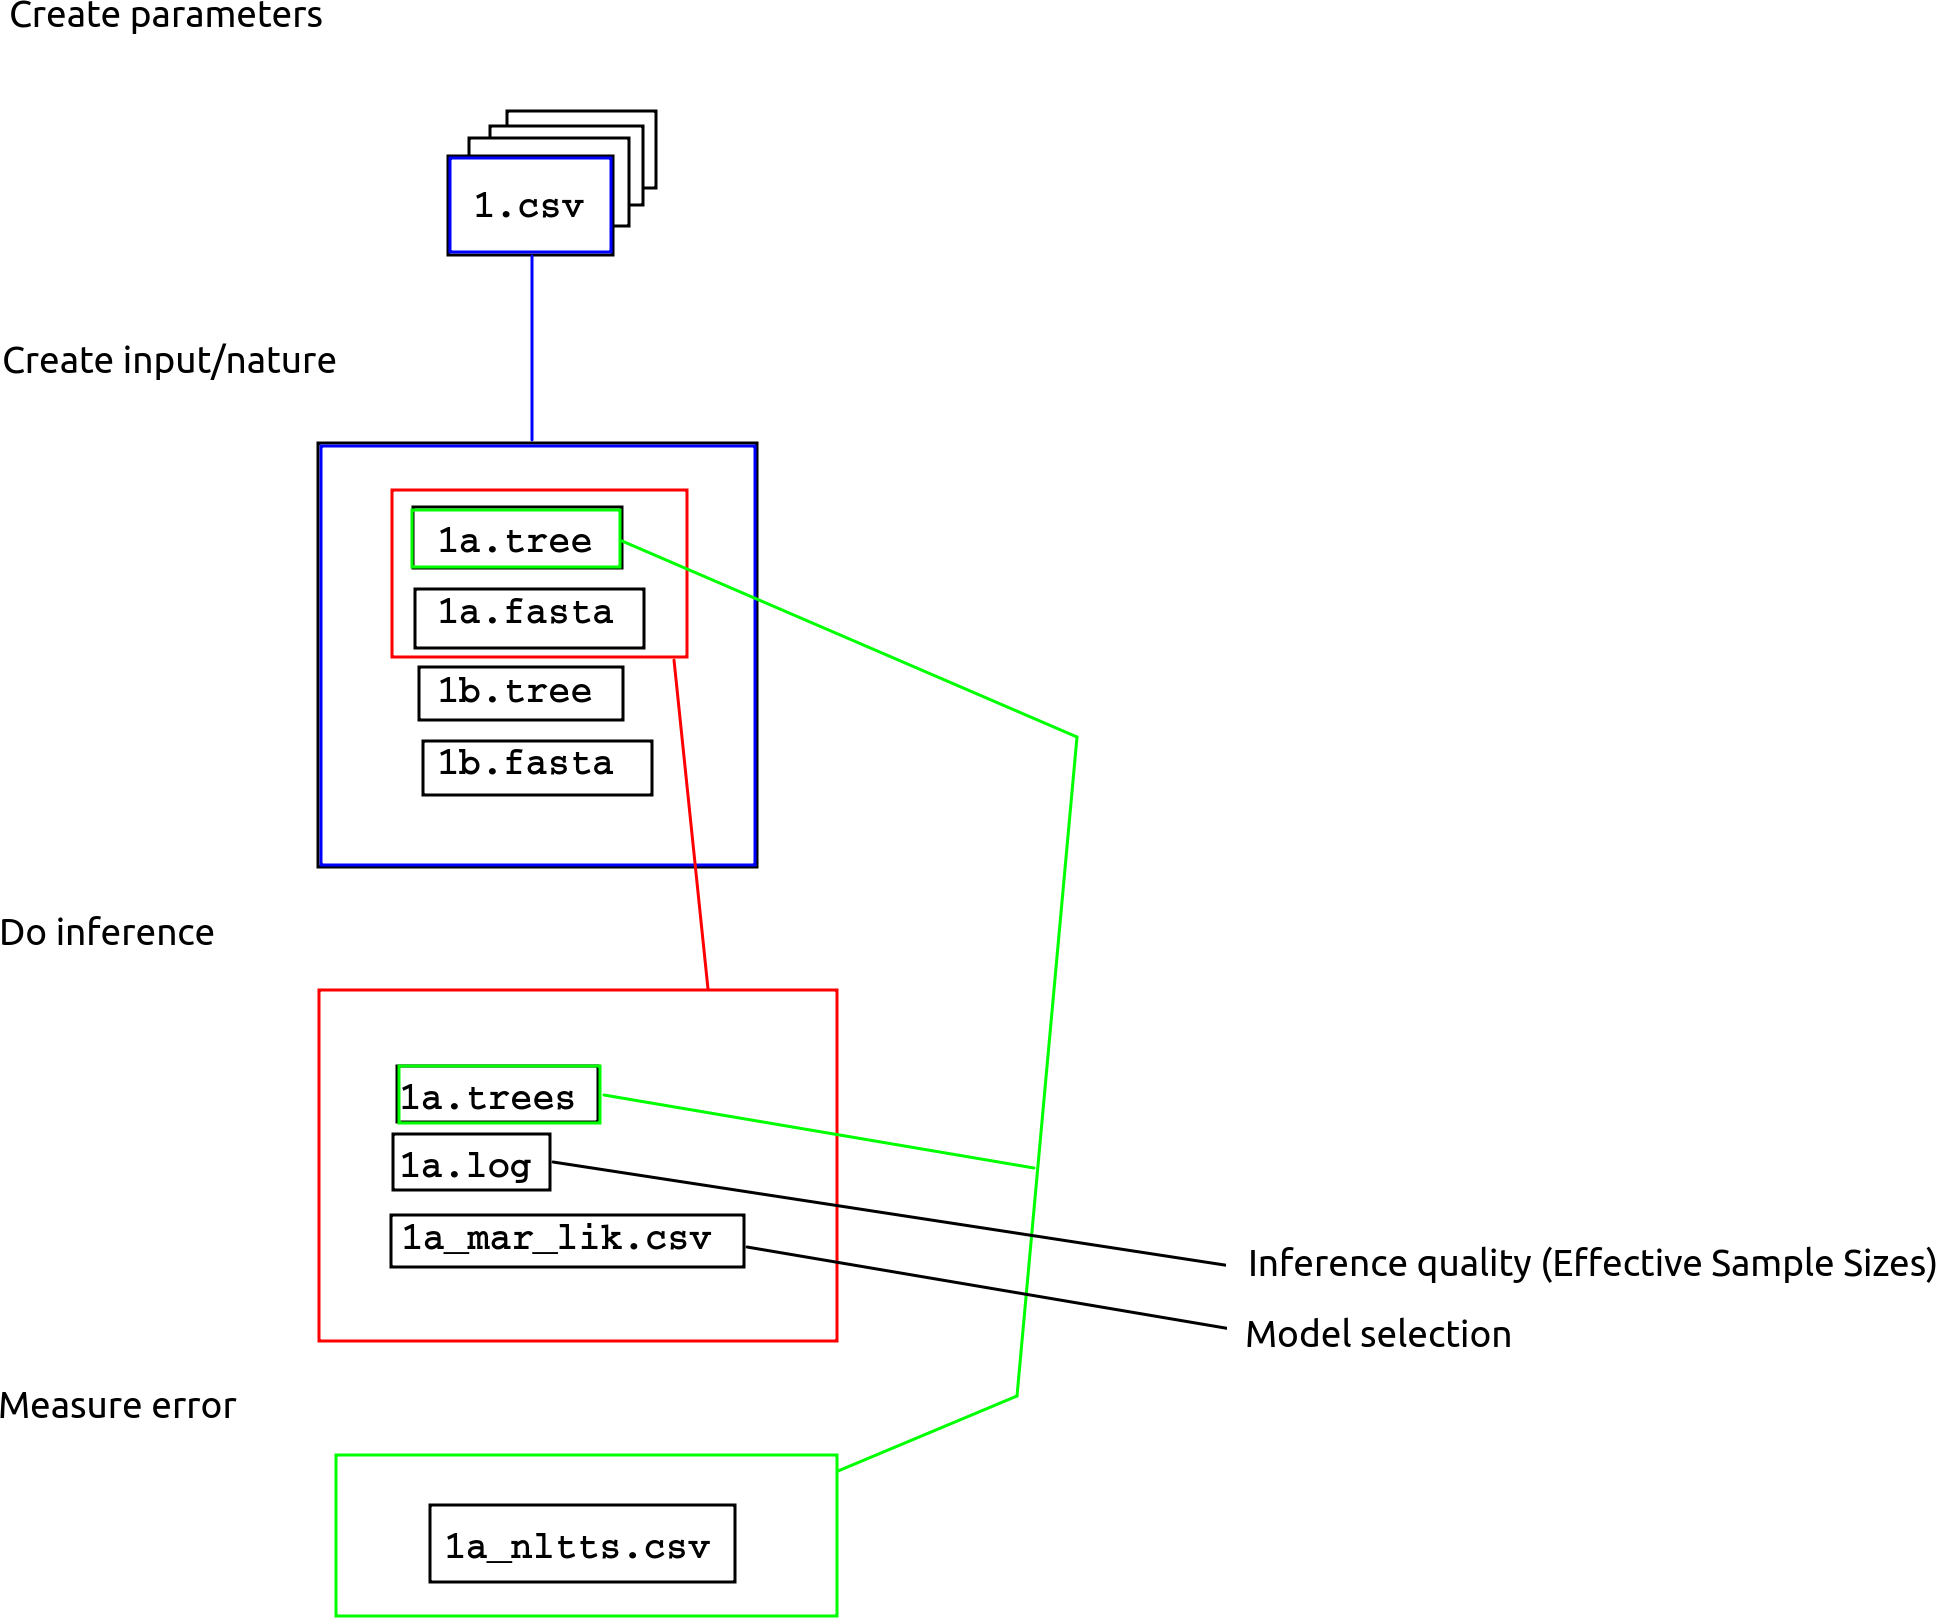
\includegraphics{pipeline.png}
\caption{Pipeline}
\end{figure}

Update our dependencies:

\begin{Shaded}
\begin{Highlighting}[]
\ControlFlowTok{if}\NormalTok{ (}\DecValTok{1} \OperatorTok{==}\StringTok{ }\DecValTok{2}\NormalTok{) \{}
\NormalTok{  devtools}\OperatorTok{::}\KeywordTok{install_github}\NormalTok{(}\StringTok{"Giappo/mbd"}\NormalTok{, }\DataTypeTok{quiet =} \OtherTok{TRUE}\NormalTok{)}
\NormalTok{  devtools}\OperatorTok{::}\KeywordTok{install_github}\NormalTok{(}\StringTok{"richelbilderbeek/beautier"}\NormalTok{, }\DataTypeTok{quiet =} \OtherTok{TRUE}\NormalTok{)}
\NormalTok{  devtools}\OperatorTok{::}\KeywordTok{install_github}\NormalTok{(}\StringTok{"richelbilderbeek/tracerer"}\NormalTok{, }\DataTypeTok{quiet =} \OtherTok{TRUE}\NormalTok{)}
\NormalTok{  devtools}\OperatorTok{::}\KeywordTok{install_github}\NormalTok{(}\StringTok{"richelbilderbeek/beastier"}\NormalTok{, }\DataTypeTok{quiet =} \OtherTok{TRUE}\NormalTok{)}
\NormalTok{  devtools}\OperatorTok{::}\KeywordTok{install_github}\NormalTok{(}\StringTok{"richelbilderbeek/mauricer"}\NormalTok{, }\DataTypeTok{quiet =} \OtherTok{TRUE}\NormalTok{)}
\NormalTok{  devtools}\OperatorTok{::}\KeywordTok{install_github}\NormalTok{(}\StringTok{"richelbilderbeek/babette"}\NormalTok{, }\DataTypeTok{quiet =} \OtherTok{TRUE}\NormalTok{)}
\NormalTok{\}}
\end{Highlighting}
\end{Shaded}

Load the library:

\begin{Shaded}
\begin{Highlighting}[]
\KeywordTok{library}\NormalTok{(razzo)}
\end{Highlighting}
\end{Shaded}

We will work in this folder:

\begin{Shaded}
\begin{Highlighting}[]
\NormalTok{super_folder_name <-}\StringTok{ }\KeywordTok{tempdir}\NormalTok{()}
\NormalTok{project_folder_name <-}\StringTok{ }\KeywordTok{file.path}\NormalTok{(super_folder_name, }\StringTok{"razzo_project"}\NormalTok{) }
\KeywordTok{dir.create}\NormalTok{(}\DataTypeTok{path =}\NormalTok{ project_folder_name, }\DataTypeTok{recursive =} \OtherTok{TRUE}\NormalTok{)}
\end{Highlighting}
\end{Shaded}

\subsection{Step 1: Create parameter
files}\label{step-1-create-parameter-files}

Here we create all parameter files:

\begin{Shaded}
\begin{Highlighting}[]
\NormalTok{parameters_filenames <-}\StringTok{ }\KeywordTok{raz_create_parameters_files}\NormalTok{(}
  \DataTypeTok{project_folder_name =}\NormalTok{ project_folder_name}
\NormalTok{)}
\end{Highlighting}
\end{Shaded}

To speed things up, we'll be keeping only two parameter files:

\begin{Shaded}
\begin{Highlighting}[]
\NormalTok{parameters_filenames <-}\StringTok{ }\NormalTok{parameters_filenames[}\KeywordTok{c}\NormalTok{(}\DecValTok{1}\NormalTok{, }\DecValTok{2}\NormalTok{)]}
\NormalTok{knitr}\OperatorTok{::}\KeywordTok{kable}\NormalTok{(parameters_filenames)}
\end{Highlighting}
\end{Shaded}

\begin{longtable}[]{@{}l@{}}
\toprule
x\tabularnewline
\midrule
\endhead
C:\Users\P274829\AppData\Local\Temp\RtmpGcGLgg/razzo\_project/data/0.2-0.15-1-0.1/1/parameters.csv\tabularnewline
C:\Users\P274829\AppData\Local\Temp\RtmpGcGLgg/razzo\_project/data/0.2-0.15-1-0.1/2/parameters.csv\tabularnewline
\bottomrule
\end{longtable}

\subsection{Step 2: create MBD trees}\label{step-2-create-mbd-trees}

\begin{Shaded}
\begin{Highlighting}[]
\NormalTok{mbd_tree_filenames <-}\StringTok{ }\NormalTok{parameters_filenames}
\CommentTok{# Create all true trees, true alignments and their twins}
\ControlFlowTok{for}\NormalTok{ (i }\ControlFlowTok{in} \KeywordTok{seq_along}\NormalTok{(parameters_filenames)) \{}
\NormalTok{  parameters_filename <-}\StringTok{ }\NormalTok{parameters_filenames[i]}
\NormalTok{  mbd_tree_filenames[i] <-}\StringTok{ }\KeywordTok{raz_create_mbd_tree_file}\NormalTok{(parameters_filename)}
\NormalTok{\}}
\end{Highlighting}
\end{Shaded}

Taking a look at the first MBD tree:

\begin{Shaded}
\begin{Highlighting}[]
\NormalTok{ape}\OperatorTok{::}\KeywordTok{plot.phylo}\NormalTok{(ape}\OperatorTok{::}\KeywordTok{read.tree}\NormalTok{(}\DataTypeTok{file =}\NormalTok{ mbd_tree_filenames[}\DecValTok{2}\NormalTok{]))}
\end{Highlighting}
\end{Shaded}

\includegraphics{razzo_pipeline_files/figure-latex/unnamed-chunk-7-1.pdf}

\subsection{Step 3: create twin BD
trees}\label{step-3-create-twin-bd-trees}

Then we want to generate a ``twin'' BD tree. To create such tree we have
to estimate the best lambda and mu to make the comparison fair. To
estimate the parameters we run a ML inference using the BD model. We
also want to condition on the same amount of tips and on the survival of
the phylogeny (cond = 2).

\begin{Shaded}
\begin{Highlighting}[]
\NormalTok{bd_tree_filenames <-}\StringTok{ }\NormalTok{parameters_filenames}
\CommentTok{# Create all BD twin trees, true alignments and their twins}
\ControlFlowTok{for}\NormalTok{ (i }\ControlFlowTok{in} \KeywordTok{seq_along}\NormalTok{(parameters_filenames)) \{}
\NormalTok{  parameters_filename <-}\StringTok{ }\NormalTok{parameters_filenames[i]}
\NormalTok{  bd_tree_filenames[i] <-}\StringTok{ }\KeywordTok{raz_create_bd_tree_file}\NormalTok{(parameters_filename)}
\NormalTok{\}}
\end{Highlighting}
\end{Shaded}

Taking a look at the first MBD tree:

\begin{Shaded}
\begin{Highlighting}[]
\NormalTok{ape}\OperatorTok{::}\KeywordTok{plot.phylo}\NormalTok{(ape}\OperatorTok{::}\KeywordTok{read.tree}\NormalTok{(}\DataTypeTok{file =}\NormalTok{ bd_tree_filenames[}\DecValTok{2}\NormalTok{]))}
\end{Highlighting}
\end{Shaded}

\includegraphics{razzo_pipeline_files/figure-latex/unnamed-chunk-9-1.pdf}

\subsection{Step 4: Create MBD
alignments}\label{step-4-create-mbd-alignments}

\begin{Shaded}
\begin{Highlighting}[]
\NormalTok{mbd_alignment_filenames <-}\StringTok{ }\NormalTok{parameters_filenames}
\CommentTok{# Create all true trees, true alignments and their twins}
\ControlFlowTok{for}\NormalTok{ (i }\ControlFlowTok{in} \KeywordTok{seq_along}\NormalTok{(parameters_filenames)) \{}
\NormalTok{  parameters_filename <-}\StringTok{ }\NormalTok{parameters_filenames[i]}
\NormalTok{  mbd_alignment_filenames[i] <-}\StringTok{ }\KeywordTok{raz_create_mbd_alignment_file}\NormalTok{(parameters_filename)}
\NormalTok{\}}
\end{Highlighting}
\end{Shaded}

Taking a look at the first MBD alignment:

\begin{Shaded}
\begin{Highlighting}[]
\KeywordTok{image}\NormalTok{(ape}\OperatorTok{::}\KeywordTok{read.FASTA}\NormalTok{(}\DataTypeTok{file =}\NormalTok{ mbd_alignment_filenames[}\DecValTok{1}\NormalTok{]))}
\end{Highlighting}
\end{Shaded}

\includegraphics{razzo_pipeline_files/figure-latex/unnamed-chunk-11-1.pdf}

\subsection{Step 5: Create BD
alignments}\label{step-5-create-bd-alignments}

\begin{Shaded}
\begin{Highlighting}[]
\NormalTok{bd_alignment_filenames <-}\StringTok{ }\NormalTok{parameters_filenames}
\CommentTok{# Create all true trees, true alignments and their twins}
\NormalTok{i <-}\StringTok{ }\DecValTok{1}
\ControlFlowTok{for}\NormalTok{ (i }\ControlFlowTok{in} \KeywordTok{seq_along}\NormalTok{(parameters_filenames)) \{}
\NormalTok{  parameters_filename <-}\StringTok{ }\NormalTok{parameters_filenames[i]}
\NormalTok{  bd_alignment_filenames[i] <-}\StringTok{ }\KeywordTok{raz_create_bd_alignment_file}\NormalTok{(parameters_filename)}
\NormalTok{\}}
\end{Highlighting}
\end{Shaded}

Taking a look at the first MBD alignment:

\begin{Shaded}
\begin{Highlighting}[]
\KeywordTok{image}\NormalTok{(ape}\OperatorTok{::}\KeywordTok{read.FASTA}\NormalTok{(}\DataTypeTok{file =}\NormalTok{ bd_alignment_filenames[}\DecValTok{1}\NormalTok{]))}
\end{Highlighting}
\end{Shaded}

\includegraphics{razzo_pipeline_files/figure-latex/unnamed-chunk-13-1.pdf}

\section{UP TILL HERE}\label{up-till-here}

\subsection{Step 2: create inference
files}\label{step-2-create-inference-files}

\begin{Shaded}
\begin{Highlighting}[]
\ControlFlowTok{if}\NormalTok{ (}\DecValTok{1} \OperatorTok{==}\StringTok{ }\DecValTok{2}\NormalTok{) \{}
  \CommentTok{# Do the inference. It doesn't work on Windows.}
\NormalTok{  mbd_alignment_filenames <-}\StringTok{ }\KeywordTok{list}\NormalTok{() }\CommentTok{# Search the folder}
  \ControlFlowTok{for}\NormalTok{ (i }\ControlFlowTok{in} \KeywordTok{seq_along}\NormalTok{(parameters_filenames)) \{}
\NormalTok{    parameter_filename <-}\StringTok{ }\NormalTok{parameters_filenames[i] }
\NormalTok{    mbd_alignment_filenames[[i]] <-}\StringTok{ }\KeywordTok{raz_create_mbd_posterior_files}\NormalTok{(}
\NormalTok{      parameter_filename}
\NormalTok{    )}
    \CommentTok{# Posterior trees}
\NormalTok{    testit}\OperatorTok{::}\KeywordTok{assert}\NormalTok{(}\StringTok{"1a.trees"} \OperatorTok\StringTok{ }\NormalTok{output_filenames)}
    \CommentTok{# Trace of MCMC, to estimate the Effective Sample Sizes}
\NormalTok{    testit}\OperatorTok{::}\KeywordTok{assert}\NormalTok{(}\StringTok{"1a.log"} \OperatorTok\StringTok{ }\NormalTok{output_filenames)}
    \CommentTok{# Marginal likelihood}
\NormalTok{    testit}\OperatorTok{::}\KeywordTok{assert}\NormalTok{(}\StringTok{"1a_mar_lik.csv"} \OperatorTok\StringTok{ }\NormalTok{output_filenames)}
\NormalTok{  \}}
\NormalTok{\}}
\end{Highlighting}
\end{Shaded}

\subsection{step 6: calculating nLTT statistics for MBD and
BD}\label{step-6-calculating-nltt-statistics-for-mbd-and-bd}

Finally we calculate the nLTT statistics for both posteriors related to
the original trees.

\begin{Shaded}
\begin{Highlighting}[]
\ControlFlowTok{if}\NormalTok{ (}\DecValTok{1} \OperatorTok{==}\StringTok{ }\DecValTok{2}\NormalTok{) \{}
  \CommentTok{# Create the nLTT distribution}
\NormalTok{  trees_filenames <-}\StringTok{ }\KeywordTok{c}\NormalTok{(}\StringTok{"1a.trees"}\NormalTok{) }\CommentTok{# Search the folder}
  \ControlFlowTok{for}\NormalTok{ (trees_filename }\ControlFlowTok{in}\NormalTok{ trees_filenames)}
\NormalTok{  \{}
    \ControlFlowTok{if}\NormalTok{ (}\DecValTok{1} \OperatorTok{==}\StringTok{ }\DecValTok{2}\NormalTok{) \{}
      \CommentTok{# }\AlertTok{TODO}\CommentTok{: Issue 5}
\NormalTok{      nltt_filename <-}\StringTok{ }\KeywordTok{raz_create_nltt_file}\NormalTok{(trees_filename)}
\NormalTok{      testit}\OperatorTok{::}\KeywordTok{assert}\NormalTok{(}\StringTok{"1a_nltts.csv"} \OperatorTok\StringTok{ }\NormalTok{nltt_filename)}
\NormalTok{    \}}
\NormalTok{  \}}
\NormalTok{\}}
\CommentTok{# All files are in place!}
\end{Highlighting}
\end{Shaded}

\begin{Shaded}
\begin{Highlighting}[]
\CommentTok{# }\AlertTok{TODO}\CommentTok{: plot the nLTT}
\end{Highlighting}
\end{Shaded}

\subsubsection{step 3: simulate the twin BD
tree}\label{step-3-simulate-the-twin-bd-tree}

\subsubsection{(check if the method to keep the topology is right. from
the figures it seems ok-ish. check with small
tree)}\label{check-if-the-method-to-keep-the-topology-is-right.-from-the-figures-it-seems-ok-ish.-check-with-small-tree}

Now that we have the BD equivalent parameters for a fair ``twinning'' we
can simulate a BD tree. We use ``TESS::tess.sim.taxa.age'' to generate
the branching times (BD\_brts). We then plug these branching times in
the l\_table coming from the original MBD tree to be sure that the
topology is the same.

\subsubsection{step 4: generate MBD posterior, given BD
prior}\label{step-4-generate-mbd-posterior-given-bd-prior}

The next step is to use the package ``pirouette'' to generate, from the
MBD tree, first the alignments and then, through BEAST, a posterior
distribution of trees. These trees are obtained using a BD prior. This
means that there are no simultaneous branching events.

\subsubsection{step 5: generate BD posterior, given BD
prior}\label{step-5-generate-bd-posterior-given-bd-prior}

\subsubsection{(check BD\_substitution rate, see Rampal's
email)}\label{check-bd_substitution-rate-see-rampals-email}

We repeat the same process for the tree simulated according to the BD
model. We want to have, in principle, the same amount of substitutions;
to do so we modify the mutation rate according to the ratio of the total
branch lenghts of the trees simulated with the two models.

\begin{Shaded}
\begin{Highlighting}[]
\ControlFlowTok{if}\NormalTok{ (}\DecValTok{1} \OperatorTok{==}\StringTok{ }\DecValTok{2}\NormalTok{) \{}
\NormalTok{  graphics}\OperatorTok{::}\KeywordTok{par}\NormalTok{(}\DataTypeTok{mfrow =} \KeywordTok{c}\NormalTok{(}\DecValTok{1}\NormalTok{, }\DecValTok{2}\NormalTok{))}
  \KeywordTok{hist}\NormalTok{(}\KeywordTok{unlist}\NormalTok{(MBD_df.nLTT), }\DataTypeTok{main =} \StringTok{"MBD nLTT"}\NormalTok{)}
  \KeywordTok{hist}\NormalTok{(}\KeywordTok{unlist}\NormalTok{(BD_df.nLTT), }\DataTypeTok{main =} \StringTok{"BD nLTT"}\NormalTok{)}
  \KeywordTok{cat}\NormalTok{(}\StringTok{"Average nLTT for MBD"}\NormalTok{, MBD_mean.nLTT, }\StringTok{"}\CharTok{\textbackslash{}n}\StringTok{Average nLTT for BD "}\NormalTok{, BD_mean.nLTT)}
\NormalTok{\}}
\end{Highlighting}
\end{Shaded}


\end{document}
